This section describes the theoretical formalism which predicts the transverse emittance growth in the presence of $\CC$ RF noise. First, it introduces the concept of noise in accelerator beam dynamics. The second section focuses on the $\CC$ noise both in amplitude and phase and it provides the equations with which one can estimate the noise-induced emittance growth. The last section comments briefly on the experiments that were carried out in KEKB: the work at KEKB constitutes the only experimental study of the effect of crab cavity RF noise prior to the work performed on SPS 



%You need the frist section to introduce the dipole noise as you will apply it in the simulations.
\section{Noise}\label{sec:noise_definition}
%External noise means that it is independent of the beam itself.
In particle accelerators, a major issue of concern is the presence noise in a variety of components used to control or observe the beam behaviour. Random fluctuations in the electric and magnetic fields seen by the beam can lead to emittance growth, orbit instability, and in extreme cases, particle loss. Examples of noise sources are ripples in the power converters which leads to fluctuations of the magnetic fields, ground motion, and various instruments in the accelerator structure such as the transverse damper and the Crab Cavities. % sofias's thesies introduction of chatper 5.
%Ripples in the power supply voltage are converted into current ripples, depending on the magnet's impedance, which eventually leads to magnetic field perturbations through the magnet's transfer function (vacuum chamber, beam screen). sofia's thesis p.95

%if you need to add references for losses etc, ref[3] of last ipac paper, even tough its for CC only.
\textbf{Emittance growth}\\
The thesis focuses on the problem of noise-induced emittance growth which has been studied extensively in the past. Past studies (theoretical and numerical) that are most relevant to the work presented in this thesis can be found in Refs.~\cite{Lebedev:248620, Lebedev:248622, PhysRevSTAB.18.101001}. In principle, if the spectrum of the noise, overlaps with the sidebands of the betatron frequencies, $(k \pm Q_u) \frev$ (where $k$ is an integer, $Q_u$ is the transverse betatron tune with $u=(x,y)$ denote the horizontal and vertical plane respectively, and $\frev$ is the revolution frequency), it drives coherent betatron oscillations. For these betatron oscillations to result in emittance growth the presence of tune spread is required. The mechanism behind the emittance growth is that the tune spread leads to a phase mixing of the particles within the bunch causing decoherence of the betatron oscillations which then results in emittance growth~\cite{Lebedev:248620}. It should be highlighted, that for all the studies presented in this thesis, the decoherence rate is fast comparing to the growth of betatron oscillations and thus the emittance growth rate is independent of the exact value of betatron tune spread~\cite{Lebedev:248620}. Last, for machines with working points far from non-linear (high-order) betatron resonances the emittance growth is linear with time and proportional to the power spectral density of the noise spectra at the betatron frequencies, $(k \pm Q_u) \frev$, mentioned above~\cite{Lebedev:248620}. This scenario holds for the work of this thesis. The definition of the power spectral density can be found in Appendix~\ref{ch:app_B}. 
% Comment 1: The last sentence is taken from the pdf of Andy part2, p.2
% Comment 2: However, in order to provide a reference for this statemrn, conclusion p.162 in the paper of lebedev.



\textbf{White noise}\\
In the studies presented in this thesis (simulations, theoretical and experimental studies), it is considered that the beam is influenced by white noise. In signal analysis, white noise is a random signal with the same amplitude (intensity) at all the frequencies which results in a uniform power spectral density. For the computational analysis (i.e. simulation studies), it is considered that the beam is influenced by the noise once per turn~\cite{Lebedev:248620, Lebedev:248622, PhysRevSTAB.18.101001}. To this end the white noise signal is sampled at a finite number of points which are called discrete-time signals. In discrete-time, the white noise can be considered as a sequence of uncorrelated random values taken from a Gaussian distribution with zero mean and finite standard deviation. More details on the continuous and discrete time analysis and the term of the power spectral density can be found in Appendix~\ref{ch:app_B}. The definition for the standard deviation of a distribution can be found in Appendix~\ref{ch:app_A}.
% Comment on uniform vs constant (Andy): "uniform" might be better than "constant".  ("constant" suggests "not changing in time", whereas here, the amplitude should be the same across a wide frequency range.)



\textbf{Dipole noise}\\
From the various noise sources that are present in an accelerator, this thesis focuses on the dipolar noise and on the $\CC$ noise. Dipolar noise is the one produced by the majority of the noise sources and is constant along the bunch, i.e. all the particles are affected the same way. % this noise is also referred to as rigid noise 
On the other hand, the way the $\CC$ noise affects the particles depends on their longitudinal position within the bunch. 

In this paragraph, the modeling of dipole noise is introduced as it constitues the basics for understanding the more complex effects of $\CC$ noise. The details on the $\CC$ noise (which is the main focus of the work presented here) are discussed further in a dedicated section (see Section~\ref{sec:CC_noise_intro}). 

%Therefore, in the following the term "noise" refers to a sequence of random kicks (stochastic process) that affect the particles within a bunch by changing their transverse momentum each turn as follows.
Past studies~\cite{Lebedev:248620, Lebedev:248622} have shown that the dipole white noise can be modeled as a sequence of random kicks (stochastic process) that affect the particles within a bunch by changing their transverse momentum each turn as follows:

%have dealt with this type of noise in the context of the induced emittance growth theoretically and in simulations. It has been shown that the noise can be modeled as a sequence of random kicks (stochastic process) that affect the particles within a bunch by changing their transverse momentum each turn as follows:
\begin{equation}\label{eq:external_noise_kicks}
    u^\prime_{j+1} =  u^\prime_j + \theta_j,
\end{equation}
%\begin{equation}\label{eq:external_noise_kicks}
%    u^\prime_{j+1} =  u^\prime_j + \Delta u^\prime_j,
%\end{equation}

where $j=\{ 0,\dots N_\mathrm{turns} \}$ denotes the turn number with $N_\mathrm{turns}$ being the total number of turns that the bunch experiences the noise and $u=(x,y)$ denotes the transverse horizontal or vertical plane. The parameter $\theta_j$ corresponds to the noise kick and is the $j$th element of a set of $N_\mathrm{turns}$ samples, drawn from a Gaussian distribution (with size $N_\mathrm{turns}$ ) with mean 0 and standard deviation, $\sigma_\theta$. This way it is ensured that the noise kicks are uncorrelated.

The standard deviation $\sigma_\mathrm{noise}$ characterises the strength of the noise. As discussed in Appendix~\ref{ch:app_B} (see Eq.~\eqref{eq:psd_for_white_noise_variance}) for a white noise spectrum, it is related to it's power spectral density, $S_\theta$, at any given frequency, $f_k$ as follows: 
\begin{equation}\label{eq:psd_for_white_noise_variance_dipole}
    S_\theta(f_k) = \frac{\sigma_\theta^2 } {\frev},
 \end{equation}
where $\frev$ is the revolution frequency of the machine.

The power spectral density, $S_\theta(f_k)$, is expressed in terms of the square of the amplitude of the signal per unit frequency. As here the noise is applied in the angle co-ordinates the units of the power spectral density are $\mathrm{rad^2/Hz}$.

In this thesis, the term "noise" will refer white noise which is modeled with the above-mentioned stochastic process.

%and $\Delta u^\prime = \zeta_j A$ is the change of the transverse direction of motion (in units of radians) due to the noise. $A$ characterises the noise strength and $\zeta_j$ is the $j$th element of a drawn sample from a Gaussian distribution with mean 0, standard deviation 1 and size $N_\mathrm{turns}$, such as the kicks are uncorrelated.


% This approach will be used in the following. In th
% if it is dipole noise it is oftern written: Delta u = thera


\section{Crab Cavity noise and emittance growth}\label{sec:CC_noise_intro}
As already mentioned in the Introduction (Section~\ref{sec:motivation_outline}) the presence of noise in the $\CC$ low-level RF system is an issue of major concern for the HL-LHC project as it results in transverse emittance growth and subsequently in loss of luminosity. To this end, in 2015, P.~Baudrenghien and T.~Mastoridis developed a theoretical model~\cite{PhysRevSTAB.18.101001} which predicts this transverse emittance growth induced by $\CC$ noise focusing on the HL-LHC scenario. In particular, the model assumes a hadron machine, zero synchrotron radiation damping, long bunches (in the order of cm), and white RF noise (discrete spectral lines are excluded). Additionally, it is assumed that the $\CC$ RF zero phase is set at the center of the bunch.

This  model is also applicable to the SPS (where the same conditions apply), where the $\CC$s will be tested before their installation in the HL-LHC (Section~\ref{sec:motivation_outline}). The equations and formulas from the theoretical model that are essential for the understanding of the studies are discussed below.

 % Thus, the results from the SPS $\CC$ tests can be used for scaling to the HL-LHC case.

\subsection{Crab Cavity amplitude and phase noise}\label{subsec:AN_PN}
The unperturbed instantaneous $\CC$ voltage equals the one of an ideal oscillator:
\begin{equation}\label{eq:CC_voltage_t}
    V_\mathrm{CC}(t) = \CCvoltage \sin{\left ( 2 \pi \CCfrequency t \right )},
\end{equation}

where $\CCvoltage$ is the peak amplitude of the $\CC$ voltage and $\CCfrequency$ the $\CC$ frequency. Equation~\eqref{eq:CC_voltage_t} can be re-written as a function of the longitudinal position within the bunch $z$ instead of time $z$ as follows:
\begin{equation}\label{eq:CC_voltage_z}
    V_\mathrm{CC}(z) = \CCvoltage \sin{\left ( \frac{2\pi \CCfrequency}{\beta_0 c}z \right )},
\end{equation}
where $\beta_0$ is the relativistic parameter and $c$ is the speed of light. The above equation is obtained as: $z=v \cdot t \Rightarrow t=z/v=z/(\beta_0 c)$.
In the presence of modulations in amplitude and phase Eq.~\eqref{eq:CC_voltage_z} becomes (details in Appendix~\ref{app:Measured_noise}):
\begin{equation}\label{eq:CC_voltage_z}
    V_\mathrm{CC}(z) = \CCvoltage (1+\Delta A) \sin{\left ( \frac{2\pi \CCfrequency}{\beta_0 c}z + \Delta \phi \right )},
\end{equation}

where $\Delta \phi$ is the deviation from the nominal phase, $2\pi \CCfrequency z/(\beta_0 c)$, and will be referred to as phase noise in the following. $\Delta A = \Delta \CCvoltage / \CCvoltage$ is the relative deviation from the nominal amplitude $\CCvoltage$ and will be referred to as amplitude noise. The units of $\Delta \phi$ is radians while $\Delta A$ has no units as it defines a scaling factor applied to the amplitude, rather than stating directly the change in the amplitude.
% Note on the above paragraph: source that ΔA = ΔV/V: https://www.osti.gov/servlets/purl/1846026/
% The units of ΔΑ and Δφ are shown in Table II of the paper of Themis and Philippe.


In the calculation of the RF noise effects it is assumed that RF phase and amplitude noises are independent. The validity of this hypothesis depends on the actual architecture of the LLRF responsible for the regulation of the cavity field. This is presently being designed at CERN. Further details can be found in Ref.~[15] of the above-mentioned publication of P.~Baudrenghien and T.~Mastoridis~\cite{PhysRevSTAB.18.101001}, but discussing them is out of the scope of this thesis.
 
%Due to the $\CC$ RF noise sources in the LHC, HL-LHC and, SPS machines, the amplitude and phase noise spectra can be considered  independent, and thus they can be treated separetatly. The technical details can be found in Ref.~[15] of the above-mentioned publication of Baudrenghien and Mastoridis~\cite{PhysRevSTAB.18.101001}, but discussing them is out of the scope of this thesis.
% 1) You need to understand Ref.[15]
% 2) Q and I demodulator --> it enables easily extracting instantaneous amplitude and phase over time. source: https://indico.cern.ch/event/781242/contributions/3251767/attachments/1780299/2896017/Powerpoint_1.pdf
% 3) Document on the digital Q/I demodulator, that might be useful when you try to understand it. https://accelconf.web.cern.ch/p95/ARTICLES/RPQ/RPQ02.PDF

To this end, and following the analysis in Ref.~\cite{PhysRevSTAB.18.101001} and in accordance with Eq.~\eqref{eq:external_noise_kicks} the phase and amplitude noise kicks on each particle within a bunch can be modeled as the following turn-by-turn change of the angle co-ordinate of each particle: % at the location of the CC; s=s_CC. Eq.7 in ref~\cite{PhysRevSTAB.18.101001} but for not normalised co-oridnates.
% Presetnation: https://docs.google.com/presentation/d/1Jv0Es99utlZSSg25_9oplI53A5MdPDfJSjsSneRXaV8/edit#slide=id.gbb99f3cf0a_0_65
\begin{equation}\label{eq:amplitude_noise_kick}
    \textbf{\textrm{Amplitude noise:}} \  u^\prime_{j+1} =  u^\prime_j + \frac{e \CCvoltage}{E_b} \Delta A_j \sin{\left (  \frac{2 \pi \CCfrequency}{c \beta_0}z   \right )},
  \end{equation}
  \begin{equation}\label{eq:phase_noise_kick}
      \textbf{\textrm{Phase noise:}} \ u^\prime_{j+1} =  u^\prime_j +  \frac{e \CCvoltage}{E_b} \Delta \phi_j  \cos{\left (  \frac{2 \pi \CCfrequency}{c \beta_0}z   \right )},
  \end{equation}
%\begin{equation}\label{eq:amplitude_noise_kick}
%  \textbf{\textrm{Amplitude noise:}} \  u^\prime_{j+1} =  u^\prime_j + \zeta_j A \sin{\left (  \frac{2 \pi \CCfrequency}{c \beta_0}z   \right )},
%\end{equation}
%\begin{equation}\label{eq:phase_noise_kick}
%    \textbf{\textrm{Phase noise:}} \ u^\prime_{j+1} =  u^\prime_j + \zeta_j A \cos{\left (  \frac{2 \pi \CCfrequency}{c \beta_0}z   \right )},
%\end{equation}
where $j=\{ 0,\dots N_\mathrm{turns} \}$ denotes the turn number with $N_\mathrm{turns}$ being the total number of turns that the bunch experiences the noise and $e$ is the proton charge. Furthermore, $u^\prime$, with $u=(x,y)$, is the angle co-ordinate and $z$ the longitudinal co-ordinate of each particle as defined in Eq.~\eqref{eq:particle_coordinates}, $\CCfrequency$ is the $\CC$ frequency, $c$ is the speed of light and $\beta_0$ the relativistic $\beta$. The parameters $\Delta A_j$ and $\Delta \phi_j$, are the $j$the elements of a set of $N_\mathrm{turns}$ samples, drawn from Gaussian distributions of size $N_\mathrm{turns}$ , with mean 0 and standard deviation of $\sigma_{\Delta A}$ and $\sigma_{\Delta \phi}$ respectively. A typical value of $\sigma_A$ and $\sigma_\phi$ that will be used in the simulations later is $2.7 \times 10^{-3}$.  It is reminded that $\sigma_\phi$ is expressed in radians, while $\sigma_A$ has no units.

\textbf{Disclaimer}\\

%Moreover, $A=\CCvoltage /(E_b \cdot \Delta A )$ or $A=\CCvoltage /(E_b \cdot \Delta \phi )$ the scaling factor for the strength of amplitude or phase noise respectively. The typical value of $A$ that will be used in the simulations later is $10^{-8}$. Finally, $\zeta_j$ is the $j$th element of a drawn sample from a Gaussian distribution with mean 0, standard deviation 1 and size $N_\mathrm{turns}$, such as the above kicks are uncorrelated (white noise).

% The following paragraph is inspired by what I said in the IPAC talk.
Figure~\ref{fig:amplitude_noise} and Fig.~\ref{fig:phase_noise} provide a schematic visualisation of the amplitude and phase noise respectively along with the impact of their kicks on the particles. It can be seen that in the presence of amplitude noise the head and the tail of the bunch are kicked in opposite directions which results in intra-bunch oscillations. On the other hand, in the presence of phase noise, the particles in the bunch receive kicks that are in phase. This results in a shift of the bunch centroid which basically is a dipole or mode 0 motion.

\begin{figure}[!h] % at the directory of ipac22
    \centering         
    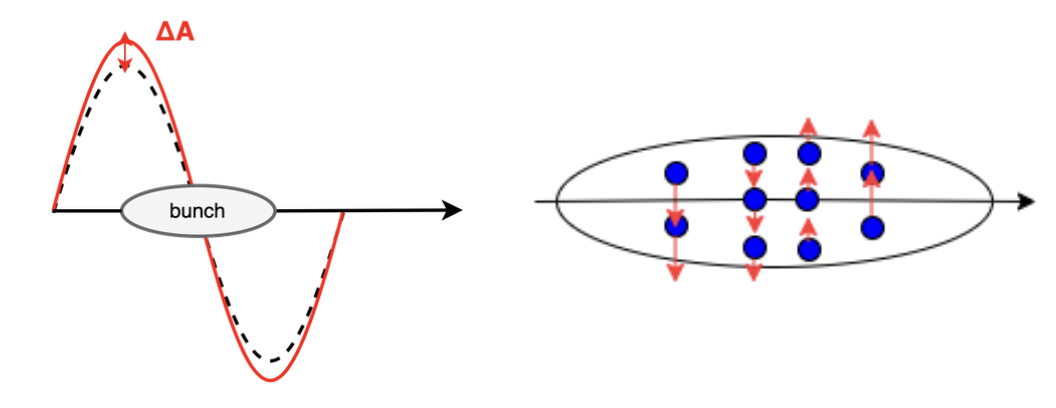
\includegraphics[width=0.8\textwidth]{images/Ch3/amplitude_noise.png}
        \caption{Modulation in amplitude or amplitude noise (left) and its impact on the particles within the bunch (right). The blue dots represent the individual particles while the red arrows indicate the direction of the noise kicks which act on them.}
        \label{fig:amplitude_noise}
 \end{figure}

 \begin{figure}[!h] % at the directory of ipac22
    \centering         
    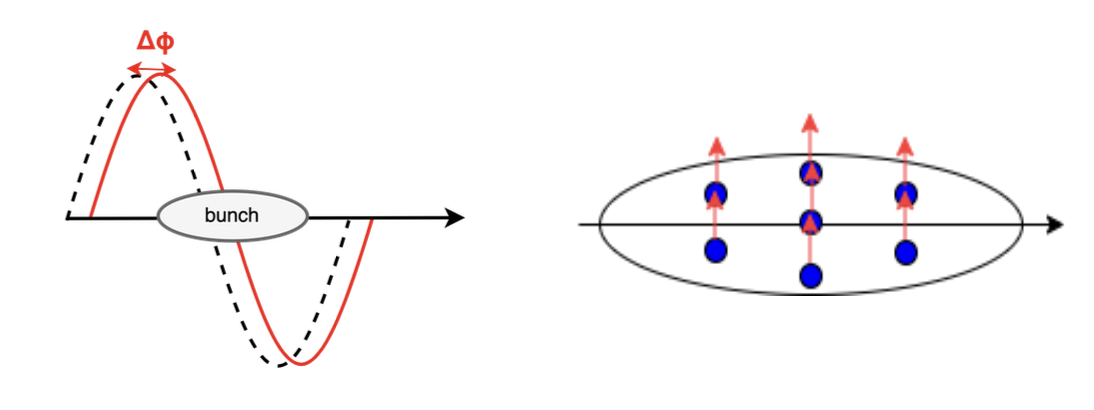
\includegraphics[width=0.85\textwidth]{images/Ch3/phase_noise.png}
        \caption{Modulation in phase or phase noise (left) and its impact on the particles within the bunch (right). The blue dots represent the individual particles while the red arrows indicate the direction of the noise kicks which act on them.}
        \label{fig:phase_noise}
 \end{figure}

 Finally, it is worth mentioning, that for the LHC, HL-LHC and SPS $\CC$s the amplitude and phase RF noise are represented by white noise spectra. In that case, they can be considered as a sequence of uncorrelated random variables taken from a Gaussian distribution with zero mean and standard deviation $\sigma_{\Delta A}$ and  $\sigma_{\Delta \phi}$ respectively which equals the total noise power (see Appendix~\ref{app:discrete_time_analysis} for definitions). % sampled by the beam, as also written here: https://www.osti.gov/servlets/purl/1846026 

\subsection{Emittance growth formulas}\label{subsec:CC_emit_growth_theoretical_formulas}
As already mentioned, the theoretical formalism for predicting the transverse emittance growth in the presence of $\CC$ RF amplitude and phase noise was derived in Ref.~\cite{PhysRevSTAB.18.101001}. The derivation assumes a single bunch, that the noise kicks are represented by a stochastic process, zero coupling between the horizontal and vertical plane, the beam energy is constant (no acceleration) and, $\CC$ RF zero phase is at the center of the bunch, $z=0$ and a uniform noise spectrum across the betatron tune distribution which is also symmetric in negative and positive frequencies. 
% One more assumption that I didn't write Inthe analysis presented in this work, the density function is independent of time (paper of themis and philippe p.2) i didn't write it in the assumption.

Taking these conditions into account, the emittance growth resulting from amplitude noise is estimated from:
\begin{equation}\label{eq:dey_an}
    \frac{d\epsilon^{\mathrm{geom}}_u}{dt}  = \beta_{u, \mathrm{CC}} \left( \frac{e\CCvoltage\frev}{2E_b}\right)^2 \!\! C_{\Delta A} (\sigma_{\phi}) \!\! \sum_{k=-\infty}^{+\infty} S_{\Delta A}[(k \pm \widebar{q}_u \pm \widebar{q}_s)\frev].
\end{equation}
For phase noise, the emittance growth is estimated from:
\begin{equation}\label{eq:dey_pn}
    \frac{d\epsilon^{\mathrm{geom}}_u}{dt}  = \beta_{u, \mathrm{CC}}  \left( \frac{e\CCvoltage\frev}{2E_b}\right)^2 C_{\Delta \phi} (\sigma_{\phi}) \sum_{k=-\infty}^{+\infty} S_{\Delta \phi}[(k \pm \widebar{q}_u) \frev].
\end{equation}
In these formulas, which are valid for both transverse planes as $u=(x,y)$, $\beta_{u, \mathrm{CC}}$ is the transverse beta function at the location of the CC, $\CCvoltage$ the CC voltage, $\frev$ the revolution frequency of the beam, $E_b$ the beam energy, and $\widebar{q}_u$ and $\widebar{q}_s$ the mean of the betatron and synchrotron tune distribution \footnote{For white noise spectra the effect of noise is independent of the actual tune distribution, hence the use of the mean quantities. The generic formulas can be found in Ref.~\cite{PhysRevSTAB.18.101001}} where $q_u, q_s$ (with lower case) denote the decimal part of the betatron and synchrotron tunes respectively. $S_{\Delta A}$ and $S_{\Delta \phi}$ are the power spectral densities (PSD) of the noise at all the betatron and synchrobetatron (for the amplitude noise case) sidebands and they are expressed in units of Hz$^{-1}$ and rad$^2$Hz$^{-1}$, respectively. In particular, $k \in \mathbb{Z}$ is the harmonic number of the revolution frequency and the $\pm$ signs refer to the upper $(+)$ and lower $(-)$ sidebands at each mulitple of the revolution frequency, $k f_\mathrm{rev}$, from the betatron tune.

The definition of the power spectral density along with the fundamental terminology for the signal-processing can be found in Appendix~\ref{ch:app_B}\footnote{In the Appendix amplitude and phase noise are noted with just $\alpha$ and $\phi$, instead of $\Delta A$ and $\Delta \phi$, for simplicity.}.
$C_{\Delta A}$ and $C_{\Delta \phi}$ are correction terms to account for the bunch length:
\begin{align}
C_{\Delta A}(\sigma_{\phi}) = ~& e^{-\sigma_{\phi}^2}\sum_{l=0}^{+\infty} I_{2l+1}(\sigma_{\phi}^2),\\
C_{\Delta \phi}(\sigma_{\phi}) = ~& e^{-\sigma_{\phi}^2} \left[I_0(\sigma_{\phi}^2) + 2 \sum_{l=1}^{+\infty} I_{2l}(\sigma_{\phi}^2) \right],
\end{align}
with $\sigma_{\phi}$ the rms bunch length, in rad, with respect to the CC frequency $\CCfrequency$, and $I_n(x)$ the modified Bessel function of the first kind. 

Figure~\ref{fig:correction_term_bunch_length} illustrates the correction term for different values of bunch length for amplitude (left) and phase (right) noise. The SPS nominal bunch length used in the CC tests is shown in the orange for reference.

% Figures created using the following script: natriant/cernbox/Project_thesis/plot_bunch_length_correction_term
\begin{figure}[!ht]
    \centering
    \begin{subfigure}[t]{0.45\textwidth}
        \centering
        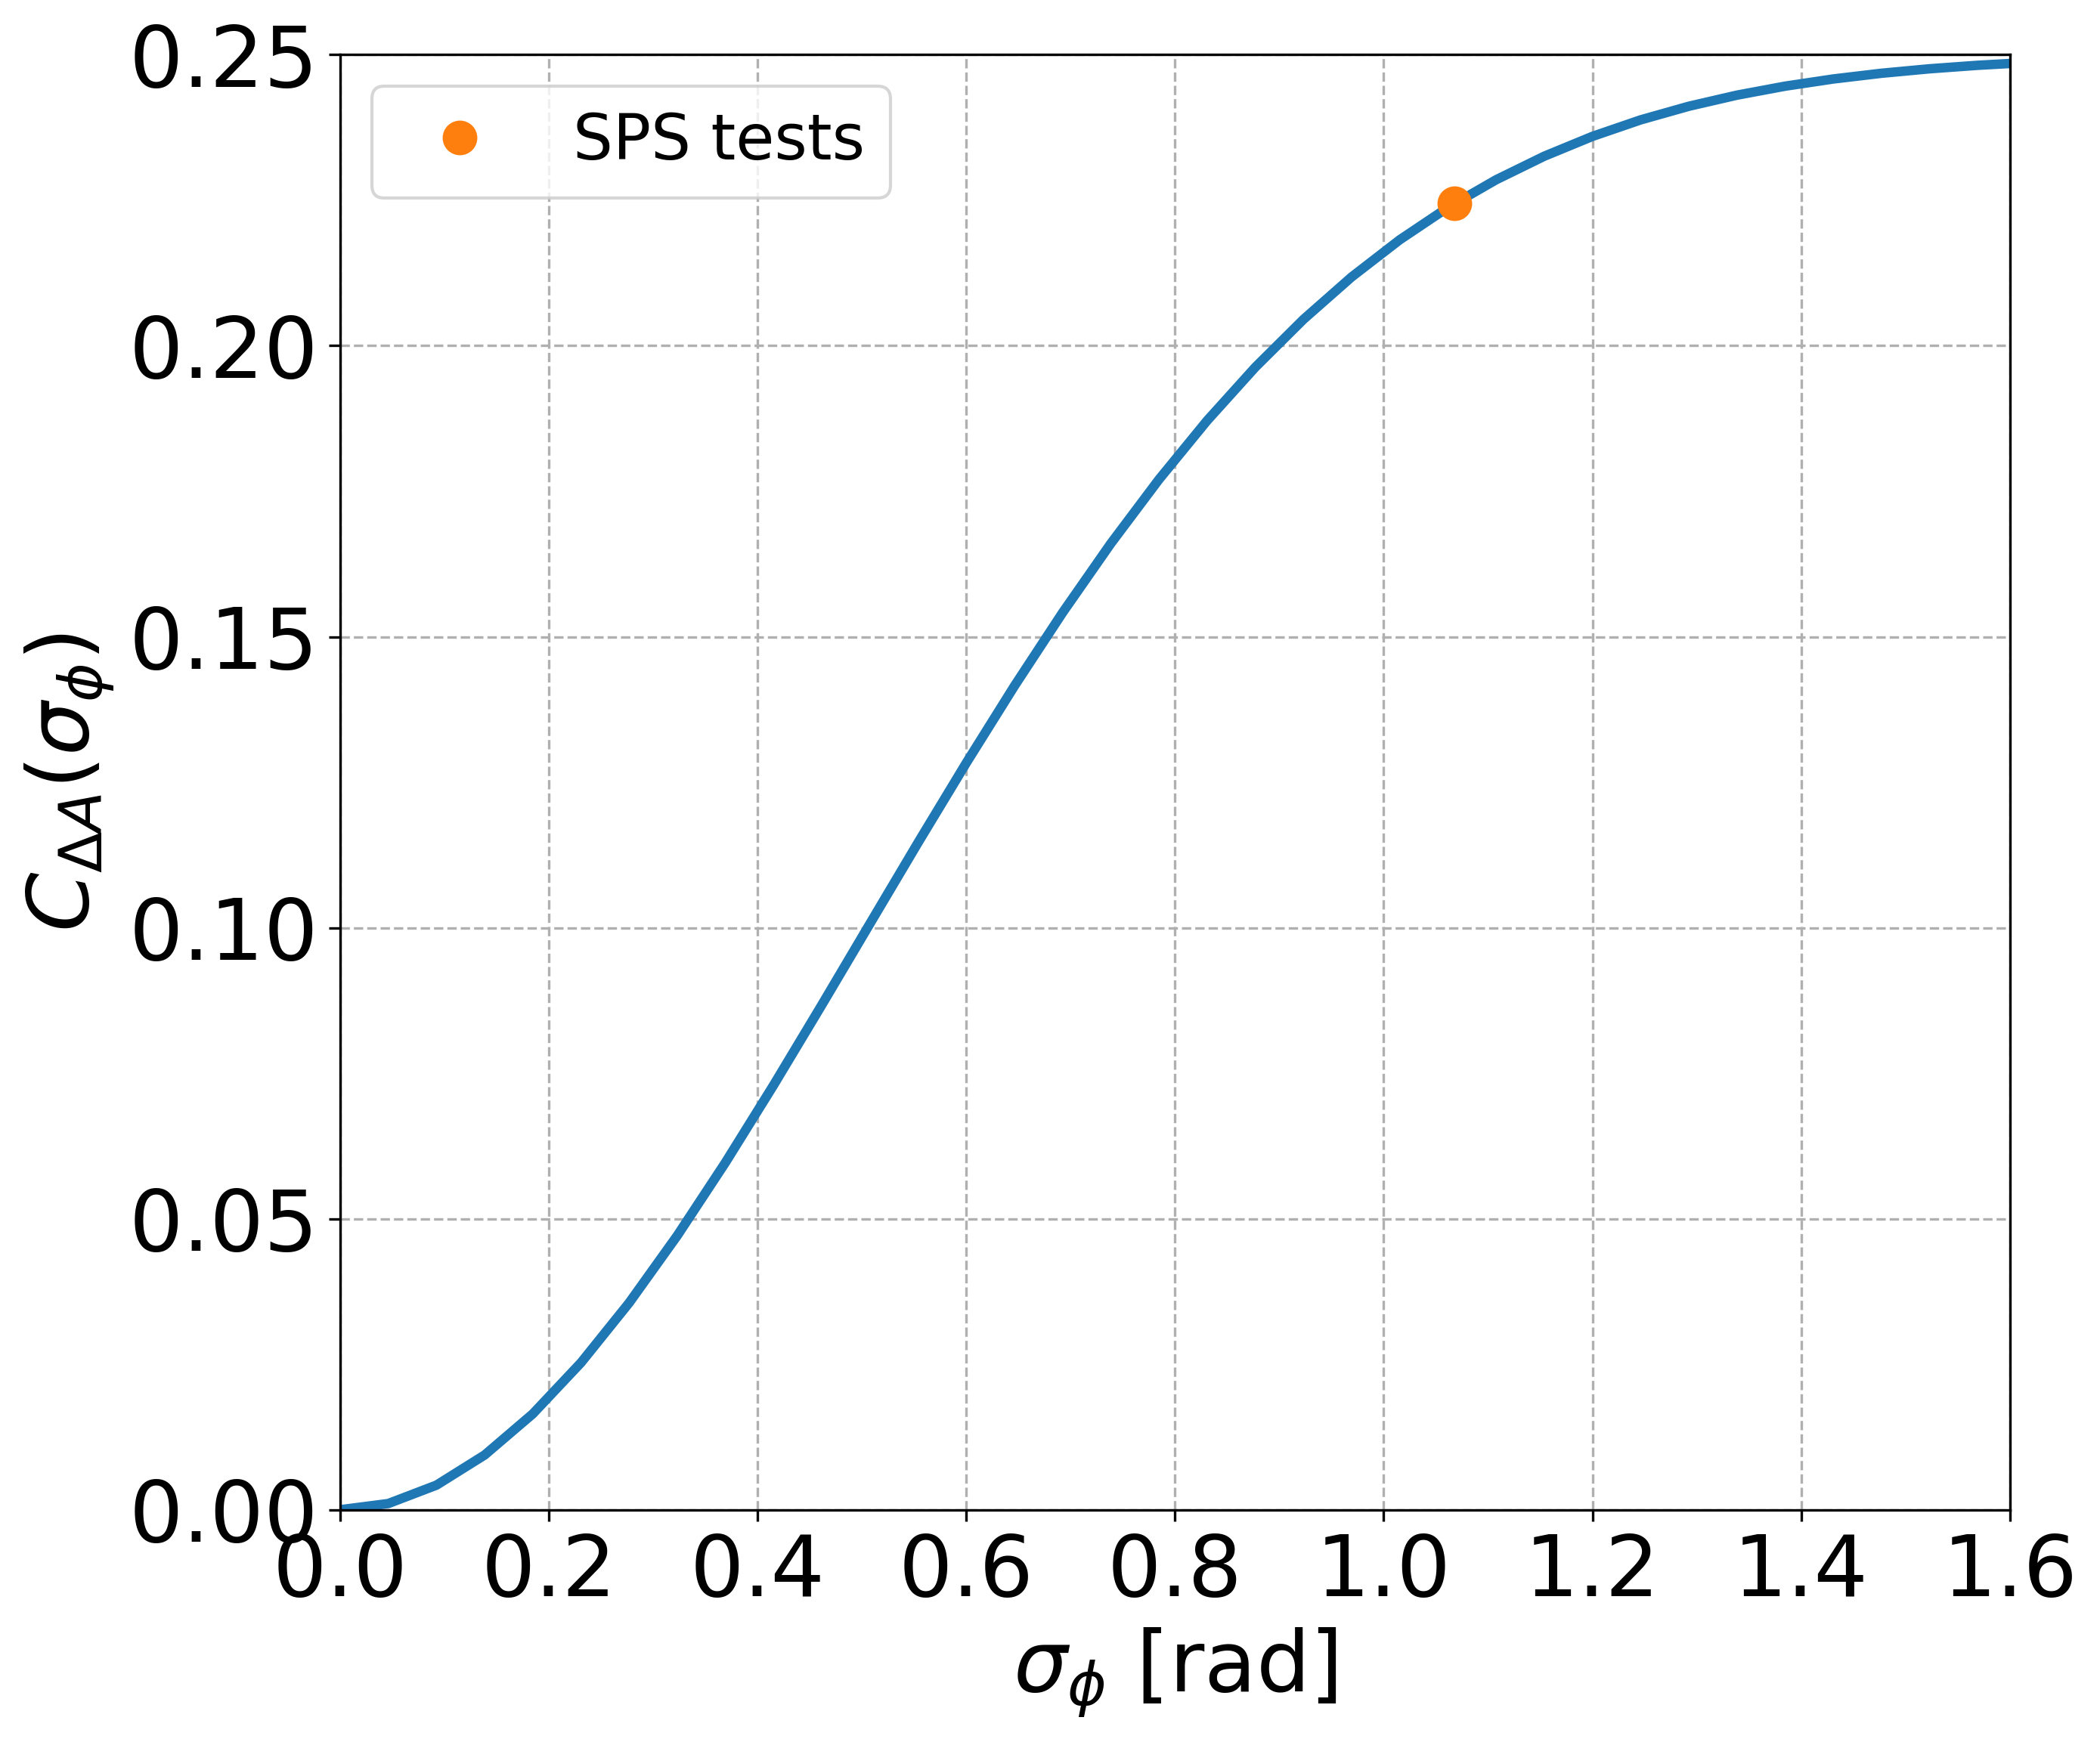
\includegraphics[width=1\textwidth]{images/Ch3/CA_bunch_length_dependence.png}
        %\caption{$y=\sin(2 \pi f t),\ f=50$ Hz}
        %\label{fig:add_label_here}
    \end{subfigure}
    \hfill
    \begin{subfigure}[t]{0.45\textwidth}
        \centering
        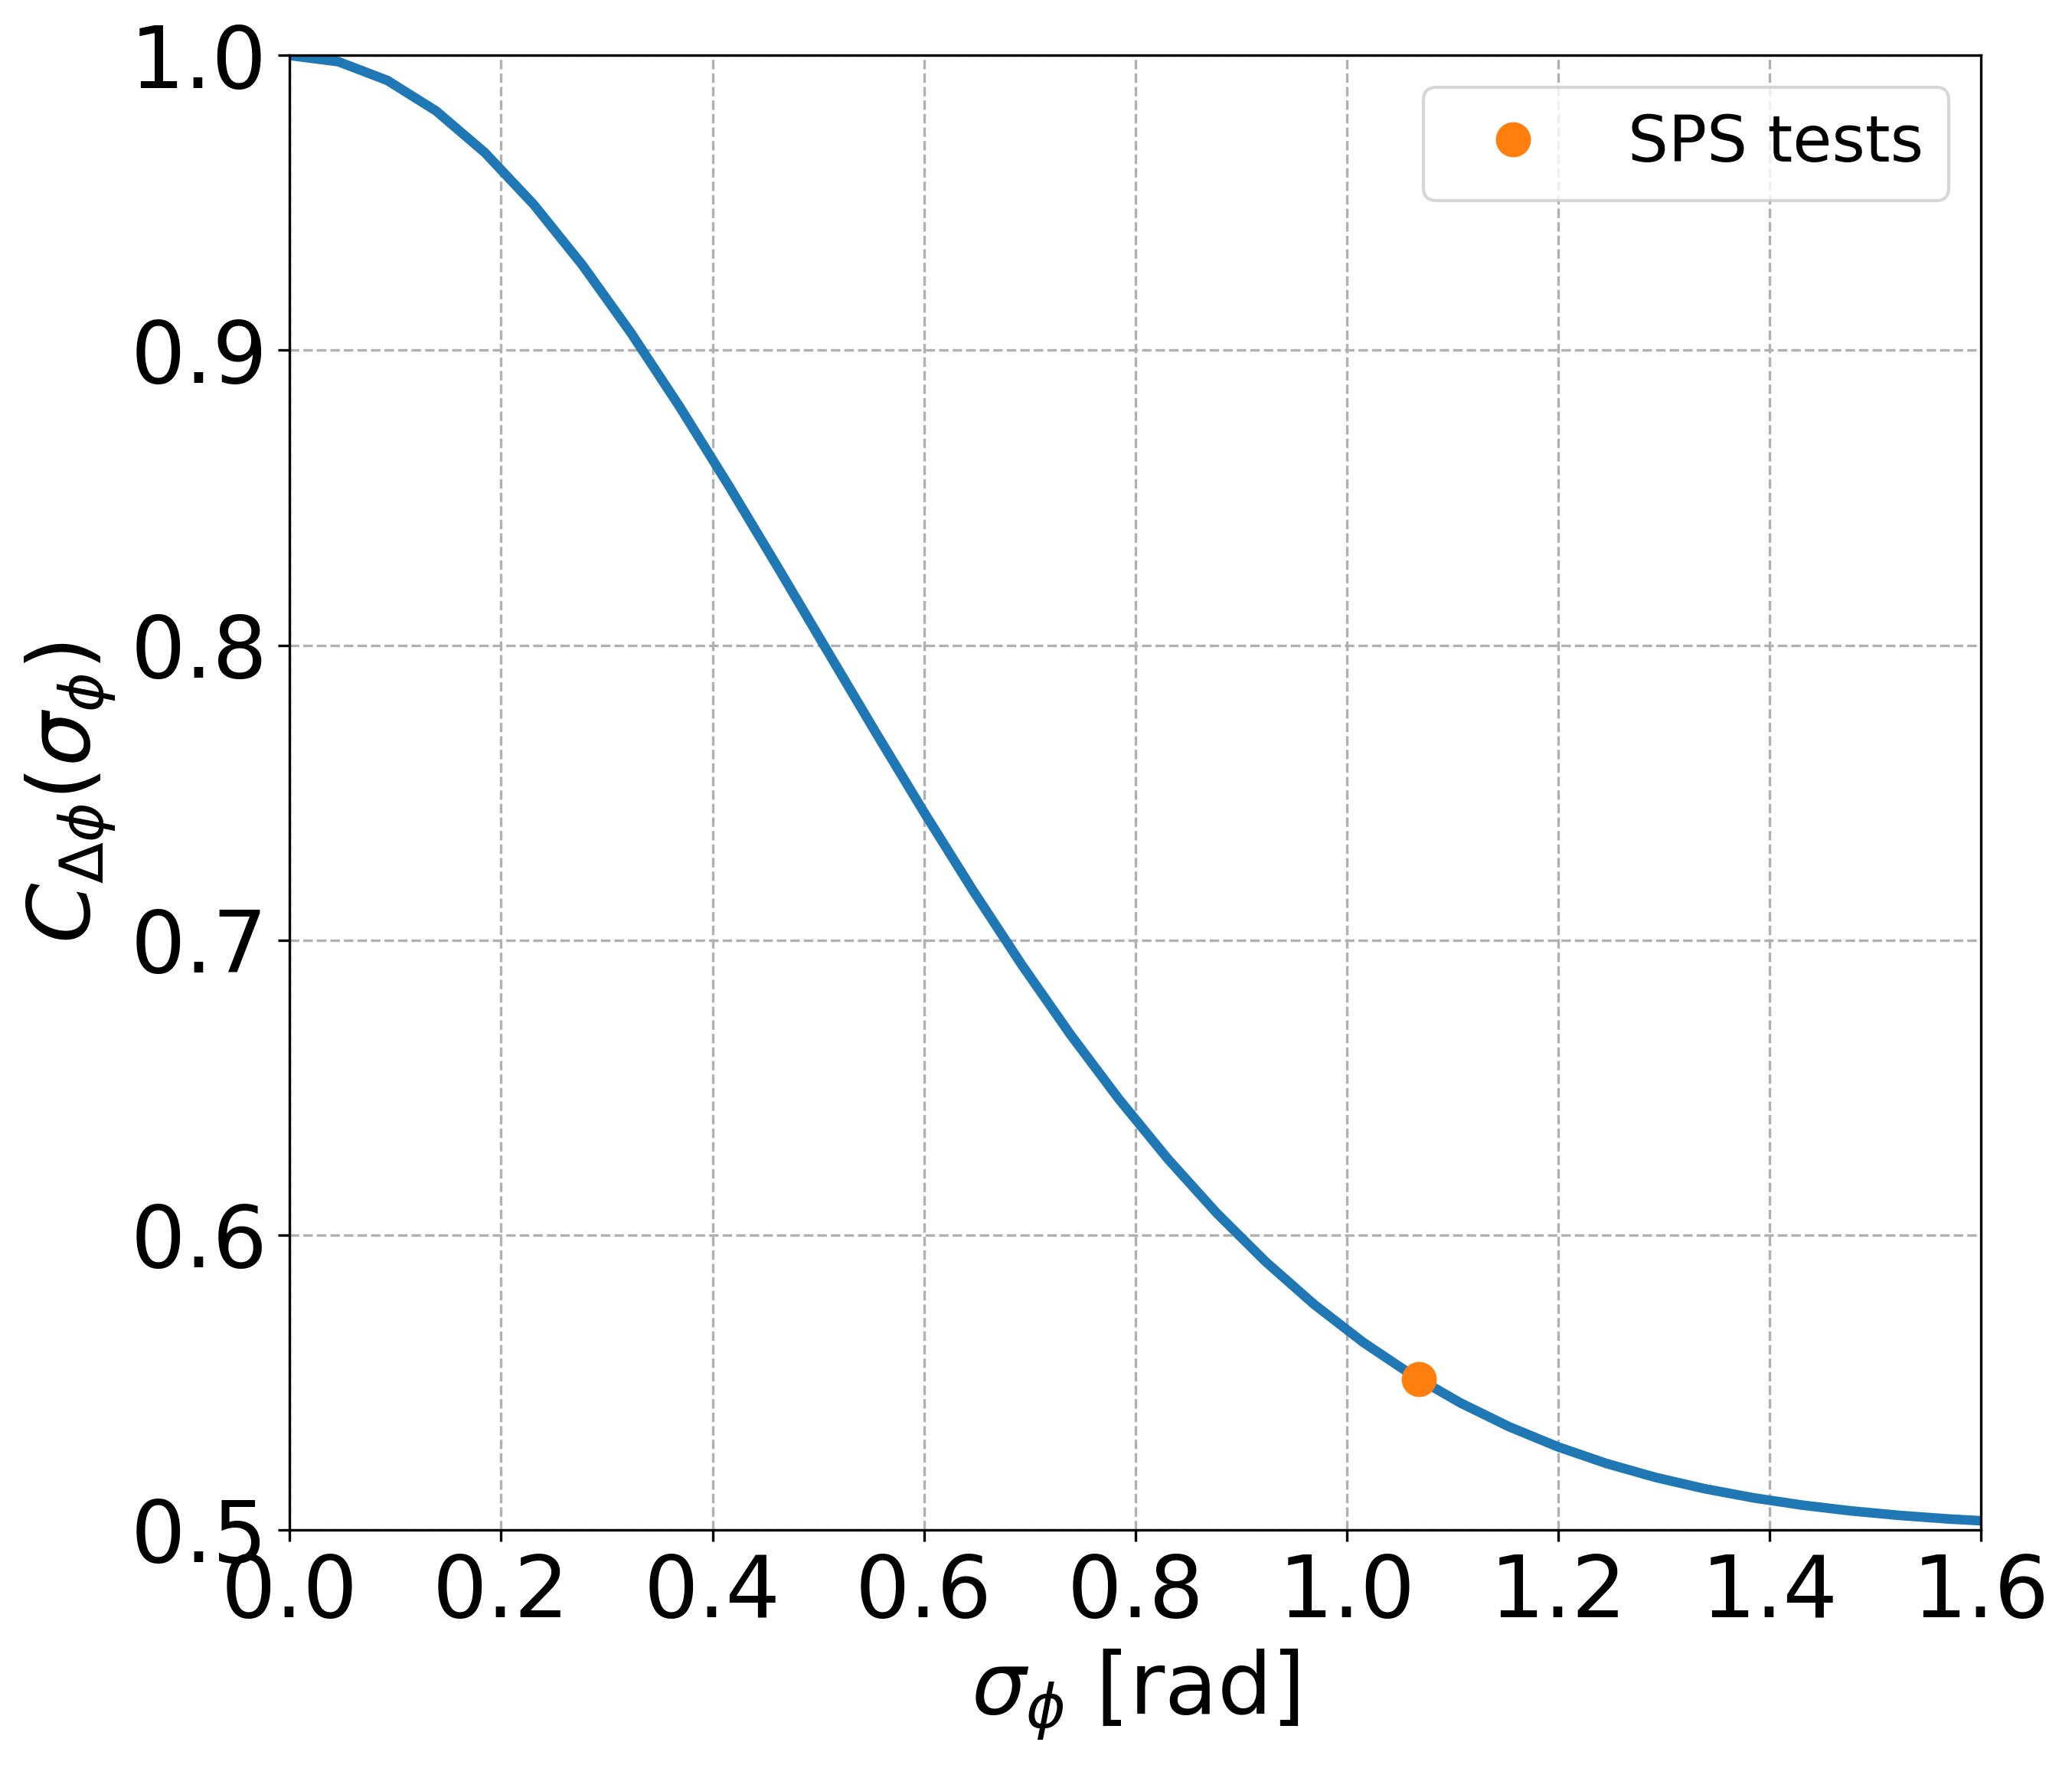
\includegraphics[width=1\textwidth]{images/Ch3/Cphi_bunch_length_dependence.png}
        %\caption{Discrete Fourier transform}
        %\label{fig:add_label_here}
    \end{subfigure}
    \hfill
     \caption{Correction term for amplitude (left) and phase (right) noise over a range of bunch length values.} % bunch passage
     \label{fig:correction_term_bunch_length}
 \end{figure}

\textbf{Comment on the use of the emittane growth formulas}\\
Here some additional comments on the use of the Eq.~\eqref{eq:dey_an} and Eq.~\eqref{eq:dey_pn} for predicting the emittance growth rate for both measurements and simulation studies of this thesis are made to facilitate the discussion in the following chapters.

In this thesis, the emittance growth in the vertical plane is addressed. The reason is that for both experimental campaigns that took place in 2018 and 2022, the $\CC$ module that was available provided a vertical deflection on the beam. For reference, the $\CC$ module which provides horizontal deflection is planned to be available by the end of 2022. Additionally the studies were performed for the SPS machine for which the parameters are listed in Table~\ref{tab:machine_beam_param_2018}: $q_y=0.18$, $f_\mathrm{rev}=43.38$\,kHz, and $q_s=0.0051$. 

To this end, the emittance growth induced by $\CC$ RF noise depends on the PSD value of the noise at the vertical betatron and synchrobetatron sidebands for the phase and amplitude noise case respectively (see Eq.~\eqref{eq:dey_an} and Eq.~\eqref{eq:dey_pn}). The upper and lower sidebands of the first and second vertical betatron sidebands are observed in the following frequencies:
\begin{equation}\label{eq:betatron_sideband_1}
    \mathrm{k=0}: \ (0 \pm \widebar{q}_y) f_\mathrm{rev} = \pm 0.18 \times 43.38\mathrm{\,kHz} \approx \pm 7.8\mathrm{\,kHz}.
\end{equation}
\begin{equation}\label{eq:betatron_sideband_2}
    \mathrm{k= \pm 1}: \ (\pm 1 \pm \widebar{q}_y) f_\mathrm{rev} = (\pm 1 \pm 0.18) \times 43.38\mathrm{\,kHz} \approx \begin{dcases*} 
        \text{$-$51.2\,kHz and $-$35.6\,kHz,} & if  $k=-1$ \\ 
        \text{51.2\,kHz and 35.6\,kHz,} & if  $k=1$  
        \end{dcases*} .
\end{equation}

The upper and lower sidebands of the first and second vertical synchrobetatron sidebands are observed in the following frequencies:
\begin{equation}\label{eq:synchrobetatron_sideband_1}
    \mathrm{k=0}: \ (0 \pm \widebar{q}_y \pm \widebar{q}_s) f_\mathrm{rev} = (\pm 0.18 \pm 0.0051) \times 43.38\mathrm{\,kHz} \approx \pm 8.02\mathrm{\,kHz} \ \mathrm{and} \pm 7.6\mathrm{\,kHz}.
\end{equation}
\begin{equation}\label{eq:synchrobetatron_sideband_2}
    \begin{split}
    \mathrm{k= \pm 1}: \ (\pm 1 \pm \widebar{q}_y \pm \widebar{q}_s) f_\mathrm{rev} = (\pm 1 \pm 0.18 \pm 0.0051)\times 43.38\mathrm{\,kHz} \approx \\ 
    \approx \begin{dcases*} 
        \text{$-$35.35, $-$35.79, $-$50.96, $-$51.40\,kHz,} & if  $k=-1$ \\ 
        \text{35.35, 35.79, 50.96, 51.40\,kHz,} & if  $k=1$  
        \end{dcases*} .
    \end{split}
\end{equation}


The experimental studies with $\CC$s (more details in Chapter~\ref{Ch:2018_analyisis}) were conducted with an artificial noise spectrum which was up to 10\,kHz, which as it becomes clear from the Eqs.~\eqref{eq:betatron_sideband_1}-~\eqref{eq:synchrobetatron_sideband_2} is overlapping and therefore exciting only the first betatron and synchrobetatron sidebands, $k=0$ (upper and lower).

In the simulations, the beam particles encounter the phase or amplitude noise kicks once per turn (more details in Chapters~\ref{Ch:investigating_discrepancy} and~\ref{Ch:suppression_impedance}). This means that the sampling frequency of the noise spectrum in the frequency domain equals, $f_s=f_\mathrm{rev}=43.38$\,kHz. This means, that the frequency spectrum of the noise applied in the simulations extends from $-f_s/2 \approx -22$\,kHz to $+f_s/2 \approx 22$\,kHz. Further explanation can be found in Appendix~\ref{ch:app_B} and specifically in the Section~\ref{subsec:generatin_noise_kicks}. Again, from Eqs.~\eqref{eq:betatron_sideband_1}-~\eqref{eq:synchrobetatron_sideband_2} it becomes clear that the noise kicks in the simulations excite only the first betatron and synchrobetatron sidebands for $k=0$ (upper and lower).

To sum up, when using Eqs.~\eqref{eq:dey_an} and~\eqref{eq:dey_pn} to predict the emittance growth rate due to $\CC$ RF noise, $k=0$ will be considered.

\section{Studies in KEKB}\label{eq:past_studies_KEKB}
$\CC$s have been tested in the past with lepton beams in KEKB in Japan (further references on their operation are given in Refs.~\cite{CC_KEKB_4440798, Funakoshi:1955812, oide:pac07-mozaki01}). %~\cite{CC_KEKB_4440798, Funakoshi:1955812, oide:pac07-mozaki01}.
The tests included studies of the effects on the beam of RF noise in the $\CC$s. However, there were significant differences in KEKB, compared to SPS, LHC and HL-LHC In particular, the studies in KEKB were conducted for lepton bunches, rather than hadron bunches.  The bunch length in KEKB was smaller by an order of magnitude than in SPS or HL-LHC: this means that the effects of amplitude noise would be negligible in KEKB.  Furthermore, synchrotron radiation in lepton storage rings provides significant damping.  Finally, the RF noise in KEKB was characterised by a single spectral line, rather than white noise. Due to these differences, the studies at KEKB are not applicable to the studies presented in this thesis. These studies can be found in Ref.~\cite{PhysRevSTAB.14.111003}: they provide the only previous experience with crab cavity operation in storage rings, but because of the differences with SPS and HL-LHC, further details of the KEKB studies are beyond the scope of this thesis



Now that the theoretical formulas for the $\CC$ RF noise-induced emittance growth have been introduced, they will be used through the following chapters for comparison against numerical simulations and experimental measurements (in the SPS) for developing confidence in the theoretical model and its predictions for the HL-LHC.
